\documentclass[11pt,a4wide]{article}
\usepackage{verbatim}
\usepackage{listings}
\usepackage{graphicx}
\usepackage{a4wide}
\usepackage{color}
\usepackage[options]{SIunits}
\usepackage{amsmath}
\usepackage{amssymb}
\usepackage[dvips]{epsfig}
\usepackage[utf8]{inputenc}
\usepackage[OT1]{fontenc}
\usepackage{cite} % [2,3,4] --> [2--4]
\usepackage{shadow}
\usepackage{hyperref}

\setcounter{tocdepth}{2}
%
\lstset{language=c++}
\lstset{alsolanguage=[90]Fortran}
\lstset{basicstyle=\small}
\lstset{backgroundcolor=\color{white}}
\lstset{frame=single}
\lstset{stringstyle=\ttfamily}
\lstset{keywordstyle=\color{red}\bfseries}
\lstset{commentstyle=\itshape\color{blue}}
\lstset{showspaces=false}
\lstset{showstringspaces=false}
\lstset{showtabs=false}
\lstset{breaklines}

\begin{document}
\tableofcontents
\newpage
\section{The algorithm}
In order to solve the one-dimensional Poisson equation
\begin{equation}
-u''(x)=f(x)
\label{eq:1}
\end{equation}
with Dirichlet boundary conditions in the interval $(0,1)$ we rewrite the latter as a set of linear equations by discretizing the problem. In this way we obtain a set of $n$ grid points with the gridwidth $h=1/(n+1)$.Then we approximate the second derivative $u''(x)$ with
\begin{equation}
-\dfrac{-v_{i+1}-v_{i-1}+2v_i}{h^2}=f_i\qquad \text{for}\; i=1,..,n
\label{eq:2}
\end{equation}
If we now multiply these equations with $h^2$ and consider the boundary conditions \mbox{$v_0=v_{n+1}=0$} we obtain a set of equations that can be written as follows:
\begin{equation}
 \begin{matrix}
2v_1 & - v_2 &          &               &          &=h^2f_1 \\
 -v_1 & +2v_2 & -v_3  &               &          &=h^2f_2 \\
         &  -v_2 & +2v_3 & -v_4       &          & =h^2f_3\\
...\\ 
         &           &          & -v_{n-1}& +2v_n & =h^2f_n\\
 \end{matrix}
\label{eq:2.2}
\end{equation}
From these $n$ equations we can easily derive the following $n\times n$-matrix equation:
\begin{equation}
     \left(\begin{array}{cccccc}
                           2& -1& 0 &\dots   & \dots &0 \\
                           -1 & 2 & -1 &0 &\dots &\dots \\
                           0&-1 &2 & -1 & 0 & \dots \\
                           & \dots   & \dots &\dots   &\dots & \dots \\
                           0&\dots   &  &-1 &2& -1 \\
                           0&\dots    &  & 0  &-1 & 2 \\
                      \end{array} \right)\left(\begin{array}{c}
                           v_1\\
                           v_2\\
                           \dots \\
                          \dots  \\
                          \dots \\
                           v_{n}\\
                      \end{array} \right)
  =\left(\begin{array}{c}
                           h^2f_1\\
                           h^2f_2\\
                           \dots \\
                           \dots \\
                          \dots \\
                           h^2f_{n}\\
                      \end{array} \right).
\label{N}\end{equation}
A more general form of the above is:
\begin{equation}
    \left(\begin{array}{cccccc}
                           a_0& b_0 & 0 &\dots   & \dots &\dots \\
                           c_1 & a_1 & b_1 &\dots &\dots &\dots \\
                           & c_2 & a_2 & b_2 & \dots & \dots \\
                           & \dots   & \dots &\dots   &\dots & \dots \\
                           &   &  &c_{n-2}  &a_{n-2}& b_{n-2} \\
                           &    &  &   &c_{n-1} & b_ {n-1}\\
                      \end{array} \right)\left(\begin{array}{c}
                           v_0\\
                           v_1\\
                           \dots \\
                          \dots  \\
                          \dots \\
                           v_{n-1}\\
                      \end{array} \right)
  =\left(\begin{array}{c}
                           w_0\\
                           w_1\\
                           \dots \\
                           \dots \\
                          \dots \\
                           w_{n-1}\\
                      \end{array} \right).
											\label{M}
\end{equation}
Since the Gaussian elimination would of course lead to the correct results here, the execution time can be easily reduced from $\sim n^3$ to $\sim n$ by applying an algorithm that no longer requires the matrix but uses the three diagonals as arrays. In other words we consider that the rest of the matrix is 0 everywhere except for these diagonals which the brute force Gaussian elimination way does not take in account. The following steps have then to be taken:
\begin{enumerate}
	\item  The three diagonals are stored in arrays $a[\;],\,b[\;],$ and $c[\;]$, as well as the right side of the equation is stored in an array $w[\;]$ of the size $n$. $c[0]$ and $b[n-1]$ are set to 0.
	\item	Then the entries in $a[\;]$ are substituted recursively by
	\begin{equation}
	\tilde{a}[0]=a[0],\quad \tilde{a}[i]=a[i]-b[i-1]\dfrac{c[i]}{\tilde{a}[i-1]}
	\label{eq:3}
	\end{equation}
	This requires $3\cdot (n-1)$ floating point operations for we obtain a division, a substraction and a multiplication for each substitution.
	\item Accordingly $w[\;]$ is substituted by
		\begin{equation}
	\tilde{w}[0]=w[0],\quad \tilde{w}[i]=w[i]-\tilde{w}[i-1]\dfrac{c[i]}{\tilde{a}[i]}
	\label{eq:4}
	\end{equation}
	This only requires $2\cdot (n-1)$ flops for we already did the division $\frac{c[i]}{\tilde{a}[i-1]}$ during the substitution above.
	\item Finally backward substitution is used to gain the result for the unknown vector $v$ which is stored in another array $v[\;]$:
		\begin{equation}
	v[n-1]=\dfrac{\tilde{w}[n-1]}{\tilde{a}[n-1]},\quad v[i]=\dfrac{\tilde{w}[i]-b[i]\cdot v[i+1]}{\tilde{a}[i-1]}
	\label{eq:5}
	\end{equation}
	This operation results in another $3\cdot(n-1)+1$ flops for we have again a substraction, a multiplication and a division for each resubstitution plus a division for the first element.
\end{enumerate}
In sum the algorithm needs $8\cdot(n-1)+1$ floating point operations to solve the general matrix equation \ref{M}. 
If we now go back to the specific marix \ref{N} we can simplify the algorithm once more by tuning the above one to our needs.  For this we go through the previous algorithm and insert the given values for the entries of the vectors $a[\;],\;b[\;]$ and $c[\;]$:
\begin{enumerate}
	\item The entries in the diagonals now are:
	\begin{equation}
	a[i]=2\quad \text{for}\; i=0,..,n-1,\quad	b[i]=-1\quad \text{for}\; i=0,..,n-2,\quad	c[i]=-1\quad \text{for}\; i=1,..,n-1
	\label{eq:6}
	\end{equation}
	In this way the array computed in \ref{eq:3} becomes a static vector that can be computed recursively once and then stored somewhere for it does not depend on the right side of the equation:
	\begin{equation}
	\tilde{a}[0]=a[0],\quad \tilde{a}[i]=a[i]-b[i-1]\dfrac{c[i]}{\tilde{a}[i-1]}=a[i]-\dfrac{1}{a[i-1]}
	\label{eq:7}
	\end{equation}
	Therefore this does require $2\cdot (n-1)$ flops -  but only once, so we can compute $\tilde{a}[\;]$ once for a very large $n$ and then make use of it for any given $w[\;]$ 
	\item Latter then is to be substituted as follows
	\begin{equation}
	\tilde{w}[0]=w[0],\quad \tilde{w}[i]=w[i]-\tilde{w}[i-1]\dfrac{c[i]}{\tilde{a}[i]}=	w[i]+\dfrac{\tilde{w}[i-1]}{\tilde{a}[i]}
	\label{eq:4}
		\end{equation}
	This requires $2\cdot(n-1)$ floating point operations.
	\item The backward substitution can then be simplified, too:
		\begin{equation}
	v[n-1]=\dfrac{\tilde{w}[n-1]}{\tilde{a}[n-1]},\quad v[i]=\dfrac{\tilde{w}[i]-b[i]\cdot v[i+1]}{\tilde{a}[i]}=\dfrac{\tilde{w}[i]+v[i+1]}{\tilde{a}[i]}
	\label{eq:5}
	\end{equation}
	This operation leads to another $2\cdot(n-1)+1$ flops.
\end{enumerate}
In sum we obtain $4\cdot(n-1)+1$ floating point operations which is more than twice as fast as the general algorithm for tridiagonal matrices. If we used standard Gaussian elemination here we would have ended up with an execution time $O(\frac{2}{3}n^3)$. An application of the LU-decomposition could have been applied but would not have been worth the effort, since - in this case - there is only one vector $w$ to be solved for. The standard LU-decomposition itself requires $O(\frac{2}{3}n^3)$ floating point operations. For solving the set of equations then we would have needed another $O(n^2)$ operations which in sum is even worse than the standard Gaussian elimination.
\section{Implementation and results}
Possible implementations of both algorithms for tridiagonal matrices are shown below, as well as the plotted results of the computations with $n=10,\;100$ and $1000$ respectively.
\begin{lstlisting}[title={solvers for tridiagonal matrices}]
double* tridiagonal (double*a, double*b, double*c, double*w, int n) 	//solves the general tridiagonal matrix
{
    double* v;
    v = new double[n];

    for (int i=1; i<n; i++)
    {
        double temp = c[i]/a[i-1];	//saves n-1 flops
        a[i] -= b[i-1]*temp;		//1.
        w[i] -= w[i-1]*temp;		//2.
    }

    v[n-1] = w[n-1]/a[n-1];		//3.		

    for (int i=n-2; i>=0; i--)
    {
        v[i] = (w[i]-b[i]*x[i+1])/a[i];
    }
    return v;
}

double* tridiagonaldiff (double* a, double* w, int n)	
//solves the discretized Poisson equation, here *a is a pointer to the static array (see 1.)
 {
    double* v;
    v = new double[n];

    for (int i=1; i<n; i++)
    {
        w[i] += w[i-1]/a[i-1];		//2.
    }

    v[n-1] = w[n-1]/a[n-1];		//3.

    for (int i = n-2; i >= 0; i--)
    {
        v[i] = (w[i]+v[i+1])/a[i];
    }
    return v;

}
\end{lstlisting}
\begin{figure}[b]
	\centering
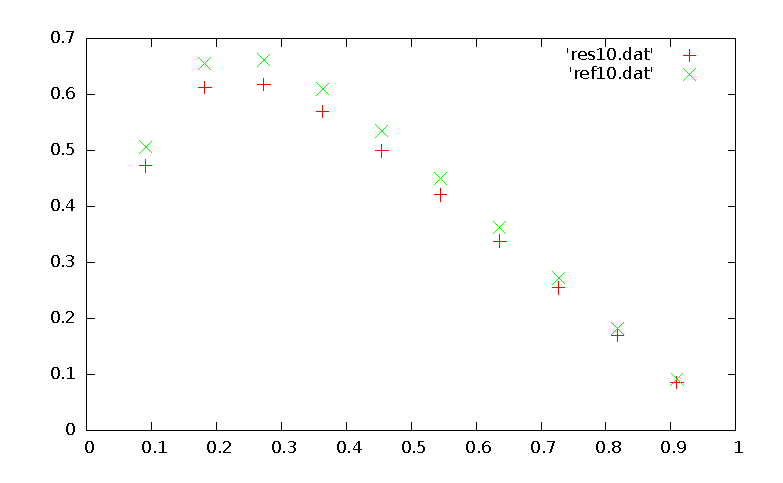
\includegraphics[scale=0.5,angle=-90]{plot10.eps}
\caption{plot with $n=10$}
	\label{fig:plot10}
\end{figure}
\begin{figure}[]
	\centering
		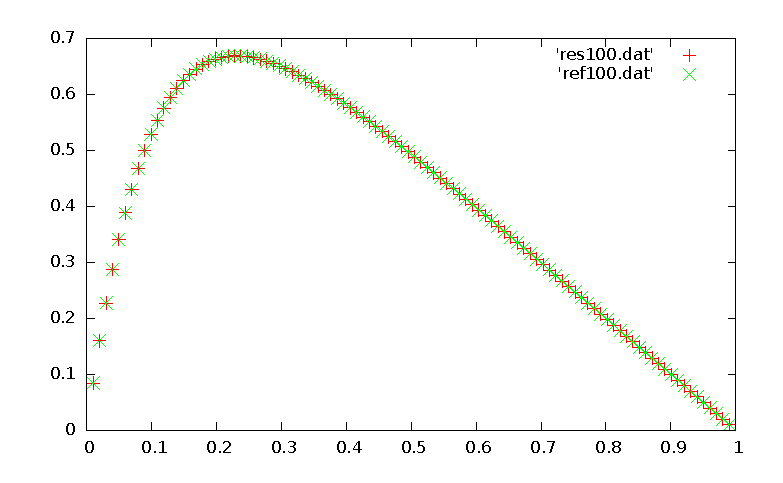
\includegraphics[scale=0.5,angle=-90]{plot100.eps}
	\caption{plot with $n=100$}
	\label{fig:plot100}
\end{figure}
\begin{figure}[]
	\centering
		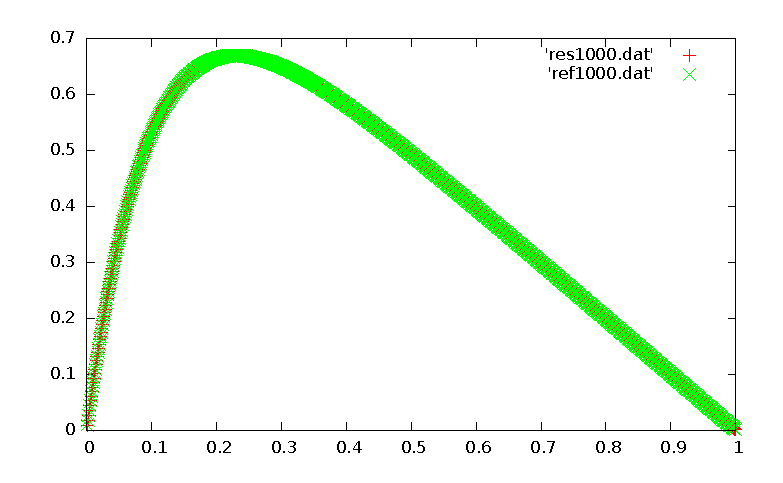
\includegraphics[scale=0.5, angle=-90]{plot1000.eps}
	\caption{plot with $n=1000$}
	\label{fig:plot1000}
\end{figure}
\section{The relative error}
The relative error $\epsilon_{i}$ for the data set $ i= 1,...,n$ is given by:
\begin{equation}
\epsilon_{i} = \log_{10}\left(\left|\dfrac{v_{i}-u_{i}}{u_{i}}\right|\right)
\end{equation}
We started with $n=10$ steps and then increased the number of steps by factor $10$ until $n=10^6$. The maximum values of the relative error for the different step lengths $h$ are shown in table \ref{tab: rel. error} and plotted in grafic \ref{graf: rel. error}.
\begin{table}[b]
\centering
\caption{max value of the relative error for different step lengths}
\label{tab: rel. error}
\begin{tabular}{lcr}\hline
	$\log10(h)$ & $\epsilon_i$ & $n$ \\
	\hline
	-1.041392685 & -1.179697782 & 10 \\
  -2.004321374 & -3.088036832 & 100 \\
  -3.000434077 & -5.080051538 & 1000 \\
  -4.000043427 & -7.079270511 & 10000 \\
  -5.000004343 & -8.847801518 & 100000 \\
  -6.000000434 & -8.05486036  & 1000000 \\	
\end{tabular}
\end{table}

\begin{figure}[t]
\centering
\label{graf: rel. error}
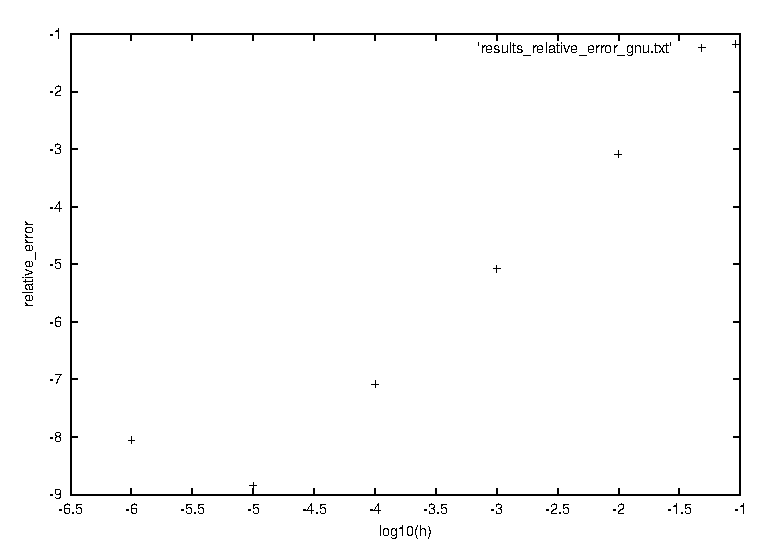
\includegraphics [scale=1] {relerr.eps}
\caption{max value of the relative error for different step lengths}
\end{figure}

When we increase the number of steps what means to reduce the step length the relative error decreases linearly (with the $\log_{10}$ scale) until $10^5$ steps. When we increase the number of steps further to $n=10^6$ the relative error becomes larger again. That shows that there is a limit to how small we can make the step length, before we run into problems with loss of precision. This also means that we can only reduce the relative error of our computed results to a certain limit.        
\section{Comparation of execution time with the LU-decomposition}
Using the LU-decomposition functions \textbf{ludcmp} and \textbf{lubskb}  given in lib.cpp to solve the Poisson equation we obtain results that are nearly identical to the results from our own algorithm. Table \ref{LUvsown} shows the relative errors between our solutions and the results from the LU decomposition. Compared to the relative error we obtain from the comparison to the reference solution one can see that the quality of both results is approximately the same since the relative error between our solution and the LU-solution is at least smaller by $3$ magnitudes than the relative error we obtain between our solution and the reference. \vspace{0.2cm}
\\ 
The comparison of execution time between the two algorithms vividly shows the importance of tuning algorithms to specific needs in order to get rid of unnecessary execution time. Table \ref{LUvsowncomp} illustrates the growth of the execution time with increasing $n$. The resolution of the timer used is about $1\milli\second$. From this we can conclude that the execution time for our linear algorithm is below $1\milli\second$ for step numbers up to $n=10^4$. For $n=10^5$ we obtain an execution time of a few milliseconds and for $n=10^6$ the time to perform the algorithm was approximately ten times longer which is exactly what we discussion in the previous paragraphs.
 \vspace{0.2cm}
\\
The LU-decomposition algorithm also behaves as expected.  For $n=10$ the execution time is smaller than the precision of the clock. But for $n=10^2$ we already get an execution time of $2\milliseconds$ and for $n=10^3$ the time rises by the factor $10^3$. This verifies the previously discussed number of flops needed for the performance of this algorithm which is $O(n^3)$. According to this the execution times for the LU-decomposition for $n=10^4$ and $n=10^5$ should rise to about $40\minute$ and $11$ days respectively. This is far beyond acceptable.
 \begin{table}%
\centering
\caption{maximum relative errors between our solution and the LU-decomposition} 
\begin{tabular}{cc}\hline
$n$ & $\epsilon_{max,n}$\\\hline
$10^1$ & -15.27 \\ 
$10^2$ & -13.91\\ 
$10^3$ & -12.41 \\ \hline
 \end{tabular}
 \label{LUvsown}
 \end{table}
 \begin{table}%
\centering
\caption{comparison of execution times between our solution and the LU-decomposition}
  \begin{tabular}{ccr}\hline
$n$ & $t$ in $\second$ for tridiagonaldiff & $t$ in $\second$ for ludcmp + lubskb \\\hline
$10^1$ & 0 & 0 \\ 
$10^2$ & 0 & 0.002 \\
$10^3$ & 0 & 2.393 \\
$10^4$ & 0 & estimated $40\minute$, too long to perform\\
$10^5$ & 0.003 & estimated $11$ days\\
$10^6$ & 0.033 & - \\
$10^7$ & 0.359 & -  \\ \hline
\end{tabular}
 \label{LUvsowncomp}
 \end{table}
\end{document}

